\documentclass[11pt,a4paper]{report}
\usepackage[utf8]{inputenc}
\usepackage[T1]{fontenc}
\usepackage{lmodern}
\usepackage{microtype}
\usepackage{graphicx}
\usepackage{hyperref}
\usepackage{listings}
\usepackage{color}
\usepackage{xcolor}
\usepackage{amsmath}
\usepackage{amssymb}
\usepackage{geometry}
\usepackage{titlesec}
\usepackage{booktabs}
\usepackage{multirow}
\usepackage{tikz}
\usetikzlibrary{shapes,arrows,positioning}

% Setup colors for code listings
\definecolor{codegreen}{rgb}{0,0.6,0}
\definecolor{codegray}{rgb}{0.5,0.5,0.5}
\definecolor{codepurple}{rgb}{0.58,0,0.82}
\definecolor{backcolour}{rgb}{0.95,0.95,0.92}

% Setup code listings
\lstdefinestyle{mystyle}{
    backgroundcolor=\color{backcolour},   
    commentstyle=\color{codegreen},
    keywordstyle=\color{magenta},
    numberstyle=\tiny\color{codegray},
    stringstyle=\color{codepurple},
    basicstyle=\ttfamily\footnotesize,
    breakatwhitespace=false,         
    breaklines=true,                 
    captionpos=b,                    
    keepspaces=true,                 
    numbers=left,                    
    numbersep=5pt,                  
    showspaces=false,                
    showstringspaces=false,
    showtabs=false,                  
    tabsize=2
}
\lstset{style=mystyle}

% Page geometry
\geometry{
    a4paper,
    total={170mm,257mm},
    left=20mm,
    top=20mm,
}

% Title format
\titleformat{\chapter}[display]
{\normalfont\huge\bfseries}{\chaptertitlename\ \thechapter}{20pt}{\Huge}
\titlespacing*{\chapter}{0pt}{50pt}{40pt}

% Document information
\title{
    \vspace{2cm}
    \Huge{Chandra Credit Software License (CCSL)} \\
    \vspace{0.5cm}
    \Large{Technical Documentation and Implementation Guide} \\
    \vspace{0.5cm}
    \large{Version 0.1.0} \\
    \vspace{2cm}
}
\author{Shyamal Chandra}
\date{May 5, 2025}

\begin{document}

\begin{titlepage}
    \maketitle
    \begin{center}
        \vfill
        \includegraphics[width=0.5\textwidth]{placeholder_logo}
        \vfill
        \large{Copyright \copyright{} 2025 Shyamal Chandra} \\
        \large{All Rights Reserved}
    \end{center}
\end{titlepage}

\tableofcontents
\newpage

\chapter{Introduction}

\section{Overview}
The Chandra Credit Software License (CCSL) is a revolutionary approach to software licensing that integrates code quality metrics with cryptocurrency micropayments. Unlike traditional licensing models that focus solely on usage rights, CCSL establishes a direct relationship between code quality, usage, and compensation.

\section{Motivation}
Software development is increasingly collaborative, yet current licensing models fail to adequately recognize and reward individual contributions based on their quality. The CCSL system aims to solve this problem by:

\begin{itemize}
    \item Objectively measuring code quality through defined metrics
    \item Enabling fair compensation proportional to contribution value
    \item Creating a more sustainable open-source ecosystem
    \item Leveraging cryptocurrency for efficient micropayments
\end{itemize}

\section{Key Components}
The CCSL system consists of three main components:

\begin{enumerate}
    \item \textbf{License Management}: Tracks code contributions and their associated metadata
    \item \textbf{Metrics Evaluation}: Evaluates code quality using six distinct metrics
    \item \textbf{Payment Integration}: Facilitates Bitcoin micropayments to contributors
\end{enumerate}

\chapter{License Management}

\section{Core Classes}
The license management component provides classes for tracking code contributions and managing license information.

\subsection{License Class}
The \texttt{License} class serves as the central point for managing a CCSL-licensed project:

\begin{lstlisting}[language=C++]
class License {
public:
    License(const std::string& projectName, const std::string& licenseKey);
    
    bool registerContribution(const CodeContribution& contribution);
    bool validate() const;
    std::string getLicenseInfo() const;
    
    // Getters
    const std::string& getProjectName() const;
    const std::string& getLicenseKey() const;
    PaymentManager& getPaymentManager();
    const std::vector<CodeContribution>& getContributions() const;
    
private:
    std::string m_projectName;
    std::string m_licenseKey;
    std::vector<CodeContribution> m_contributions;
    PaymentManager m_paymentManager;
};
\end{lstlisting}

\subsection{CodeContribution Class}
The \texttt{CodeContribution} class represents a specific contribution to the codebase:

\begin{lstlisting}[language=C++]
class CodeContribution {
public:
    CodeContribution(const std::string& contributor, 
                     const std::string& fileId,
                     int lineStart, 
                     int lineEnd);
    
    void addMetricEvaluation(const MetricEvaluation& evaluation);
    double calculateValue() const;
    
    // Getters
    const std::string& getContributor() const;
    const std::string& getFileId() const;
    std::pair<int, int> getLineRange() const;
    const std::vector<MetricEvaluation>& getMetricEvaluations() const;
    
private:
    std::string m_contributor;
    std::string m_fileId;
    int m_lineStart;
    int m_lineEnd;
    std::vector<MetricEvaluation> m_evaluations;
};
\end{lstlisting}

\subsection{PaymentManager Class}
The \texttt{PaymentManager} class handles payment tracking within a license:

\begin{lstlisting}[language=C++]
class PaymentManager {
public:
    explicit PaymentManager(const std::string& walletAddress);
    
    bool recordPayment(const CodeContribution& contribution, double amount);
    double getTotalPaymentsForContributor(const std::string& contributor) const;
    std::string generatePaymentReport() const;
    
    // Getters
    const std::string& getWalletAddress() const;
    const std::unordered_map<std::string, double>& getPayments() const;
    
private:
    std::string m_walletAddress;
    std::unordered_map<std::string, double> m_payments;
};
\end{lstlisting}

\chapter{Metrics Evaluation}

\section{Metrics Overview}
The CCSL system evaluates code quality using six distinct metrics:

\begin{table}[H]
\centering
\begin{tabular}{llp{8cm}}
\toprule
\textbf{Metric} & \textbf{Range} & \textbf{Description} \\
\midrule
Impact & 0.0 - 1.0 & Measures the gravity effect towards a particular line in the overall function of the program \\
Simplicity & 0.0 - 1.0 & Measures purity of syntactic, semantic, and pragmatic quality to be easily digested by programmers \\
Cleanness & 0.0 - 1.0 & Measures proper formatting and subsymbolic and symbolic notation \\
Comment & 0.0 - 1.0 & Measures quality of non-opinionated statements with no syntactic sugar \\
Creditability & 0.0 - 1.0 & Measures evidence that technique is compatible with architecture requirements \\
Novelty & 0.0 - 1.0 & Measures creative and exotic approach to problem-solving \\
\bottomrule
\end{tabular}
\caption{CCSL Metrics Summary}
\end{table}

\section{Metrics Structure}

\subsection{MetricType Enumeration}
The metrics are defined by the \texttt{MetricType} enumeration:

\begin{lstlisting}[language=C++]
enum class MetricType {
    IMPACT,
    SIMPLICITY,
    CLEANNESS,
    COMMENT,
    CREDITABILITY,
    NOVELTY
};
\end{lstlisting}

\subsection{MetricEvaluation Structure}
Each evaluation of a metric is represented by the \texttt{MetricEvaluation} structure:

\begin{lstlisting}[language=C++]
struct MetricEvaluation {
    MetricType type;
    double value;
    std::string rationale;
};
\end{lstlisting}

\subsection{MetricEvaluator Interface}
All metric evaluators implement the \texttt{MetricEvaluator} interface:

\begin{lstlisting}[language=C++]
class MetricEvaluator {
public:
    virtual ~MetricEvaluator() = default;
    
    virtual MetricEvaluation evaluate(const std::string& code) const = 0;
    virtual std::string getDescription() const = 0;
    virtual MetricType getType() const = 0;
};
\end{lstlisting}

\section{Implementation Details}
Each metric evaluator analyzes code to provide a score between 0.0 and 1.0:

\subsection{Impact Evaluator}
Analyzes function calls and control structures to determine how much impact the code has on the overall functionality.

\subsection{Simplicity Evaluator}
Examines factors like line length, nesting depth, and symbol density to evaluate how easily the code can be understood.

\subsection{Cleanness Evaluator}
Checks formatting consistency, indentation, and bracket style to evaluate the code's cleanliness.

\subsection{Comment Evaluator}
Analyzes comment density, quality, and relevance to assess documentation value.

\subsection{Creditability Evaluator}
Looks for evidence of testing, documentation, and external references to establish credibility.

\subsection{Novelty Evaluator}
Identifies advanced language features, design patterns, and algorithm analysis to measure innovation.

\chapter{Payment Integration}

\section{Bitcoin Integration}

The payment integration component enables Bitcoin micropayments for code contributions through the following classes:

\subsection{BitcoinPaymentManager Class}
Manages Bitcoin transactions:

\begin{lstlisting}[language=C++]
class BitcoinPaymentManager {
public:
    explicit BitcoinPaymentManager(const std::string& apiKey);
    
    bool initialize();
    std::future<std::string> sendPayment(
        const std::string& sourceWallet,
        const std::string& destinationWallet,
        double amount,
        const std::string& contributionId,
        PaymentVerificationCallback callback
    );
    bool verifyPayment(const std::string& transactionId);
    std::vector<PaymentTransaction> getTransactions() const;
    std::vector<PaymentTransaction> getTransactionsForContribution(
        const std::string& contributionId) const;
    
private:
    std::string m_apiKey;
    std::vector<PaymentTransaction> m_transactions;
};
\end{lstlisting}

\subsection{PaymentSubscription Class}
Manages recurring payment subscriptions:

\begin{lstlisting}[language=C++]
class PaymentSubscription {
public:
    PaymentSubscription(
        const std::string& contributorId,
        const std::string& walletAddress,
        int subscriptionPeriod
    );
    
    bool processPayment(BitcoinPaymentManager& paymentManager, double amount);
    bool isPaymentDue() const;
    
    // Getters
    std::string getContributorId() const;
    std::string getWalletAddress() const;
    int getSubscriptionPeriod() const;
    std::chrono::system_clock::time_point getNextPaymentDate() const;
    
private:
    std::string m_contributorId;
    std::string m_walletAddress;
    int m_subscriptionPeriod;
    std::chrono::system_clock::time_point m_nextPaymentDate;
};
\end{lstlisting}

\subsection{RecurringPaymentManager Class}
Manages multiple payment subscriptions:

\begin{lstlisting}[language=C++]
class RecurringPaymentManager {
public:
    explicit RecurringPaymentManager(BitcoinPaymentManager& paymentManager);
    
    void addSubscription(const PaymentSubscription& subscription);
    bool removeSubscription(const std::string& contributorId);
    int processDuePayments();
    const std::vector<PaymentSubscription>& getSubscriptions() const;
    
private:
    BitcoinPaymentManager& m_paymentManager;
    std::vector<PaymentSubscription> m_subscriptions;
};
\end{lstlisting}

\section{Payment Flow}
\begin{figure}[H]
\centering
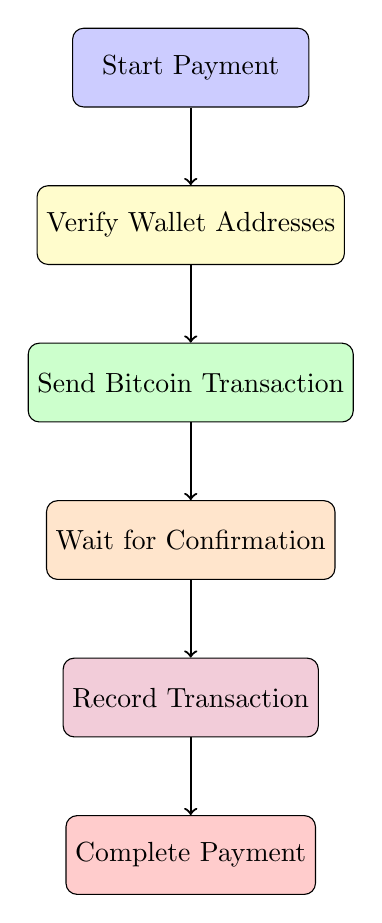
\begin{tikzpicture}[node distance=2cm]
\node (start) [rectangle, rounded corners, draw=black, fill=blue!20, minimum width=3cm, minimum height=1cm] {Start Payment};
\node (verify) [rectangle, rounded corners, draw=black, fill=yellow!20, minimum width=3cm, minimum height=1cm, below of=start] {Verify Wallet Addresses};
\node (send) [rectangle, rounded corners, draw=black, fill=green!20, minimum width=3cm, minimum height=1cm, below of=verify] {Send Bitcoin Transaction};
\node (wait) [rectangle, rounded corners, draw=black, fill=orange!20, minimum width=3cm, minimum height=1cm, below of=send] {Wait for Confirmation};
\node (record) [rectangle, rounded corners, draw=black, fill=purple!20, minimum width=3cm, minimum height=1cm, below of=wait] {Record Transaction};
\node (end) [rectangle, rounded corners, draw=black, fill=red!20, minimum width=3cm, minimum height=1cm, below of=record] {Complete Payment};

\draw[->, thick] (start) -- (verify);
\draw[->, thick] (verify) -- (send);
\draw[->, thick] (send) -- (wait);
\draw[->, thick] (wait) -- (record);
\draw[->, thick] (record) -- (end);
\end{tikzpicture}
\caption{Payment Flow Diagram}
\end{figure}

\chapter{Usage Examples}

\section{Basic Usage Example}

The following example demonstrates basic usage of the CCSL system:

\begin{lstlisting}[language=C++]
#include <ccsl/license.hpp>
#include <iostream>

using namespace ccsl;

int main() {
    // Create a license
    License license("Example Project", "CCSL-EXAMPLE-2025");
    
    // Register a contribution
    CodeContribution contribution("Alice Smith", "main.cpp", 1, 100);
    
    // Add metric evaluations
    MetricEvaluation impact;
    impact.type = MetricType::IMPACT;
    impact.value = 0.85;
    impact.rationale = "High impact code";
    
    contribution.addMetricEvaluation(impact);
    
    // Register the contribution
    license.registerContribution(contribution);
    
    // Record a payment
    license.getPaymentManager().recordPayment(contribution, 0.001);
    
    // Display license info
    std::cout << license.getLicenseInfo() << std::endl;
    
    return 0;
}
\end{lstlisting}

\section{Metrics Evaluation Example}

This example demonstrates how to evaluate code quality using the metrics system:

\begin{lstlisting}[language=C++]
#include <ccsl/metrics.hpp>
#include <iostream>

using namespace ccsl;

int main() {
    // Create code to evaluate
    std::string code = R"(
        // Calculate factorial
        int factorial(int n) {
            if (n <= 1) return 1;
            return n * factorial(n-1);
        }
    )";
    
    // Create metrics evaluator
    MetricsEvaluator evaluator;
    
    // Evaluate the code
    auto evaluations = evaluator.evaluateAll(code);
    
    // Print results
    for (const auto& eval : evaluations) {
        std::cout << "Metric: ";
        switch (eval.type) {
            case MetricType::IMPACT:      std::cout << "Impact"; break;
            case MetricType::SIMPLICITY:  std::cout << "Simplicity"; break;
            case MetricType::CLEANNESS:   std::cout << "Cleanness"; break;
            case MetricType::COMMENT:     std::cout << "Comment"; break;
            case MetricType::CREDITABILITY: std::cout << "Creditability"; break;
            case MetricType::NOVELTY:     std::cout << "Novelty"; break;
        }
        std::cout << ", Value: " << eval.value << std::endl;
        std::cout << "Rationale: " << eval.rationale << std::endl;
    }
    
    // Calculate overall value
    double value = evaluator.calculateValue(code);
    std::cout << "Overall value: " << value << std::endl;
    
    return 0;
}
\end{lstlisting}

\section{Bitcoin Payment Example}

This example demonstrates how to send Bitcoin payments for code contributions:

\begin{lstlisting}[language=C++]
#include <ccsl/payment.hpp>
#include <iostream>

using namespace ccsl;

int main() {
    // Create payment manager
    BitcoinPaymentManager manager("api-key-123");
    
    // Initialize
    if (!manager.initialize()) {
        std::cerr << "Failed to initialize payment manager" << std::endl;
        return 1;
    }
    
    // Set up payment callback
    auto callback = [](const PaymentTransaction& tx, bool success) {
        if (success) {
            std::cout << "Payment successful: " << tx.amount << " BTC" << std::endl;
        } else {
            std::cerr << "Payment failed" << std::endl;
        }
    };
    
    // Send payment
    std::future<std::string> future = manager.sendPayment(
        "1A1zP1eP5QGefi2DMPTfTL5SLmv7DivfNa",  // source
        "3J98t1WpEZ73CNmQviecrnyiWrnqRhWNLy",  // destination
        0.0005,  // amount
        "contribution-123",  // contribution ID
        callback
    );
    
    // Wait for result
    std::string txId = future.get();
    std::cout << "Transaction ID: " << txId << std::endl;
    
    return 0;
}
\end{lstlisting}

\chapter{Conclusion}

\section{Summary}
The Chandra Credit Software License (CCSL) system provides a comprehensive framework for integrating code quality metrics with cryptocurrency micropayments. By objectively measuring code quality and enabling fair compensation, CCSL aims to create a more sustainable and equitable software development ecosystem.

\section{Future Work}
Future versions of the CCSL system will include:

\begin{itemize}
    \item Integration with more cryptocurrencies beyond Bitcoin
    \item Advanced machine learning algorithms for metrics evaluation
    \item A web-based dashboard for managing licenses and payments
    \item Integration with popular version control systems
    \item Mobile applications for payment tracking and verification
\end{itemize}

\section{Final Thoughts}
The CCSL system represents a significant step toward recognizing and rewarding the true value of code contributions. By combining objective quality metrics with cryptocurrency micropayments, it offers a new model for software licensing that benefits both contributors and users.

\appendix
\chapter{License Text}
\lstinputlisting[caption=CCSL License Text]{../../license.md}

\end{document}